% !TEX root=frame_thesis.tex
\chapter{Results}

\section{Standard Run}
The standard run of the ABM presented in Section \ref{chap:Methods} aims to proof the general functioning and coherence of the model.
The simulation with parameter settings given in Table \ref{tab:sensitivity} is performed with five different seeds and the resulting mean and standard deviation of aggregated variables are shown in Figure \ref{fig:STDstats}.
The spatial patterns of tree cover, farming and settlements at different times of one single run are shown in Figure \ref{fig:STDrull}.
The results replicate in general the expected behaviour. 
In the beginning of the simulation agents settle at Anakena Beach (in the North). 
The local tree density is at the carrying capacity and thus the agents' tree preference high (blue colour).
The agents' population size grows at a constant maximum growth rate, because trees and arable land are both abundant. 
Consequently, groups of individuals split, form new agents and start to settle the rest of the island.
As Rano Kau is the major freshwater source until the end of the first drought period in $1200\, {\rm A.D.}$, new agents tend to settle in the arable coastal region South/ South East of the island in close proximity to Rano Kau with low penalties for geography, freshwater distance and farming. 
As the population density grows, deforestation and farming activity in this region intensify, and consequently agents spread out further.
After $1200\, {\rm A.D.}$, also the region around Rano Raraku, now filled with freshwater, is settled at quick pace.
%At $1200\,{\rm A.D.}$, the drought period ends and Rano Raraku (in the West) provides another freshwater source, causing many new agents to move to the South West and North West coast.
%With ever increasing population density, especially in these centres, 
Agents adapt to the slow environmental change with a linearly decreasing tree preference and, thus, intensified farming activity.
As Figure \ref{fig:STDstats} shows, the amount of burnt trees to clear land for agriculture in a 20 year time window also increases linearly until $1550\, {\rm A.D}$.
%, followed by a sharp increase around 1650.
%At peak, roughly $10\cdot 10^3$ trees are cleared in a 20 year period in order to fill the agents' farming requirement.
%The tree harvest needs of the ever growing population in the densely populated areas and, in a self-enhancing loop, the increase in burning of trees lead to further decrease of the agent's tree preference, therefore, to more land required for farming.
Thereby, agents accelerate the depletion of the non-renewable resource, trees.

Further, this large-scale deforestation leads to a sharp increase of erosion of well-suited sites around $1650\, {\rm A.D.}$ and, hence, agents need to acquire more and more farming sites.
% with the first agents not meeting their resource requirements.
However, since both no further arable sites are available in the densely populated coastal regions and trees are deforested entirely by the remaining agents, these previously well-suited regions are abandoned and the agents turn to the mostly poorly suited upland areas causing a shift towards the interior of the island.
The share farming activity on those poorly suited cells rises from a negligible fraction in $1650\, {\rm A.D.}$ to $40\%$ of all farming activity in $1700\,{\rm A.D.}$.
%With the first agents not meeting their farming requirements around 1650, occupation of upland poorly suited farming sites jumps from a negligible fraction in $1650$ to $40-59\%$ in 1700.
%Consequently, the amount of burned trees rises quickly and comes to a abrupt halt between 1700 and 1800.
Due to the low productivity indices of these sites, the use of burning trees to clear more space rises sharply in this period.

While in $1700\,{\rm A.D.}$ more than half of the agents experience some shortage in farming produce, the sudden loss of the resource trees is what sets in an exponentially decreasing mean happiness just after $1700\, {\rm A.D.}$.
This also marks the end of the net exponential growth of the population size, which peaks at around $18\cdot 10^3$ people.
Within a relative short time period of less than $50$ years, the population starts to decrease exponentially with a rate of around $-0.5$ to $-1\%$ (see Figure \ref{fig:app:STDnetgrowthrate}).
Note, that most of the agents have not enough farming sites with a happiness $H_{\rm i}(t)>H_{\rm equ}$ and therefore positive net growth. 
The agents unable to find enough trees to cut, however, at this point of time quickly vanish as there are no valid locations to settle anymore.

As the population size is decreased significantly and burning of trees stops as less aggregated farming land is required, the deforestation level slows down around $1750\, {\rm A.D.}$ with less than $25\%$ of the initial total number of trees. 

Finally, by $1800\,{\rm A.D.}$, the population decrease slows down. 
The net population growth is shown in Figure \ref{fig:app:STDnetgrowthrate}. 
There is no stable population in this model setting as tree regeneration rate is $0$ in this scenario and, hence, the agents rely on an entirely non-renewable resource.



%especially cultivation of poorly suited sites, which in turn increases the fires and amplifying the development.
%In turn, sharp increase of fires around $1600\, {\rm A.D.}$. 
%Around $1650\, {\rm A.D.}$, constant exponential growth stops, population size remains constant for a short period and, finally, decays exponentially.
%This coincides with a steep increase of agents with not enough available farming productivity causing the mean happiness to decline. 
%As shown in Figure \ref{fig:happyStd}
%However, only when trees become scarce in the region

The uncertainty of the ensemble run results from slight differences in the timing of the dynamics due to different realisations of the discrete, stochastic population growth process (see also Figure \ref{fig:realisationsofpopgrowth}.


% \begin{itemize}
% 	\item Fig 2: Aggregate Dynamics (population, trees, mean penalties and happiness, fires, excess mortality/fertility). The plot that Esteban sketched during last Zoom Meeting [called statistics plot from now on]. All statistics plots are mean ensemble runs of 5 different seeds.
% 	\item Fig 1: Comparison of the spatial deforestation pattern with \citet{Rull2020}'s Figure, which we sent to Valenti.
% \end{itemize}

\begin{figure}
	\centering
	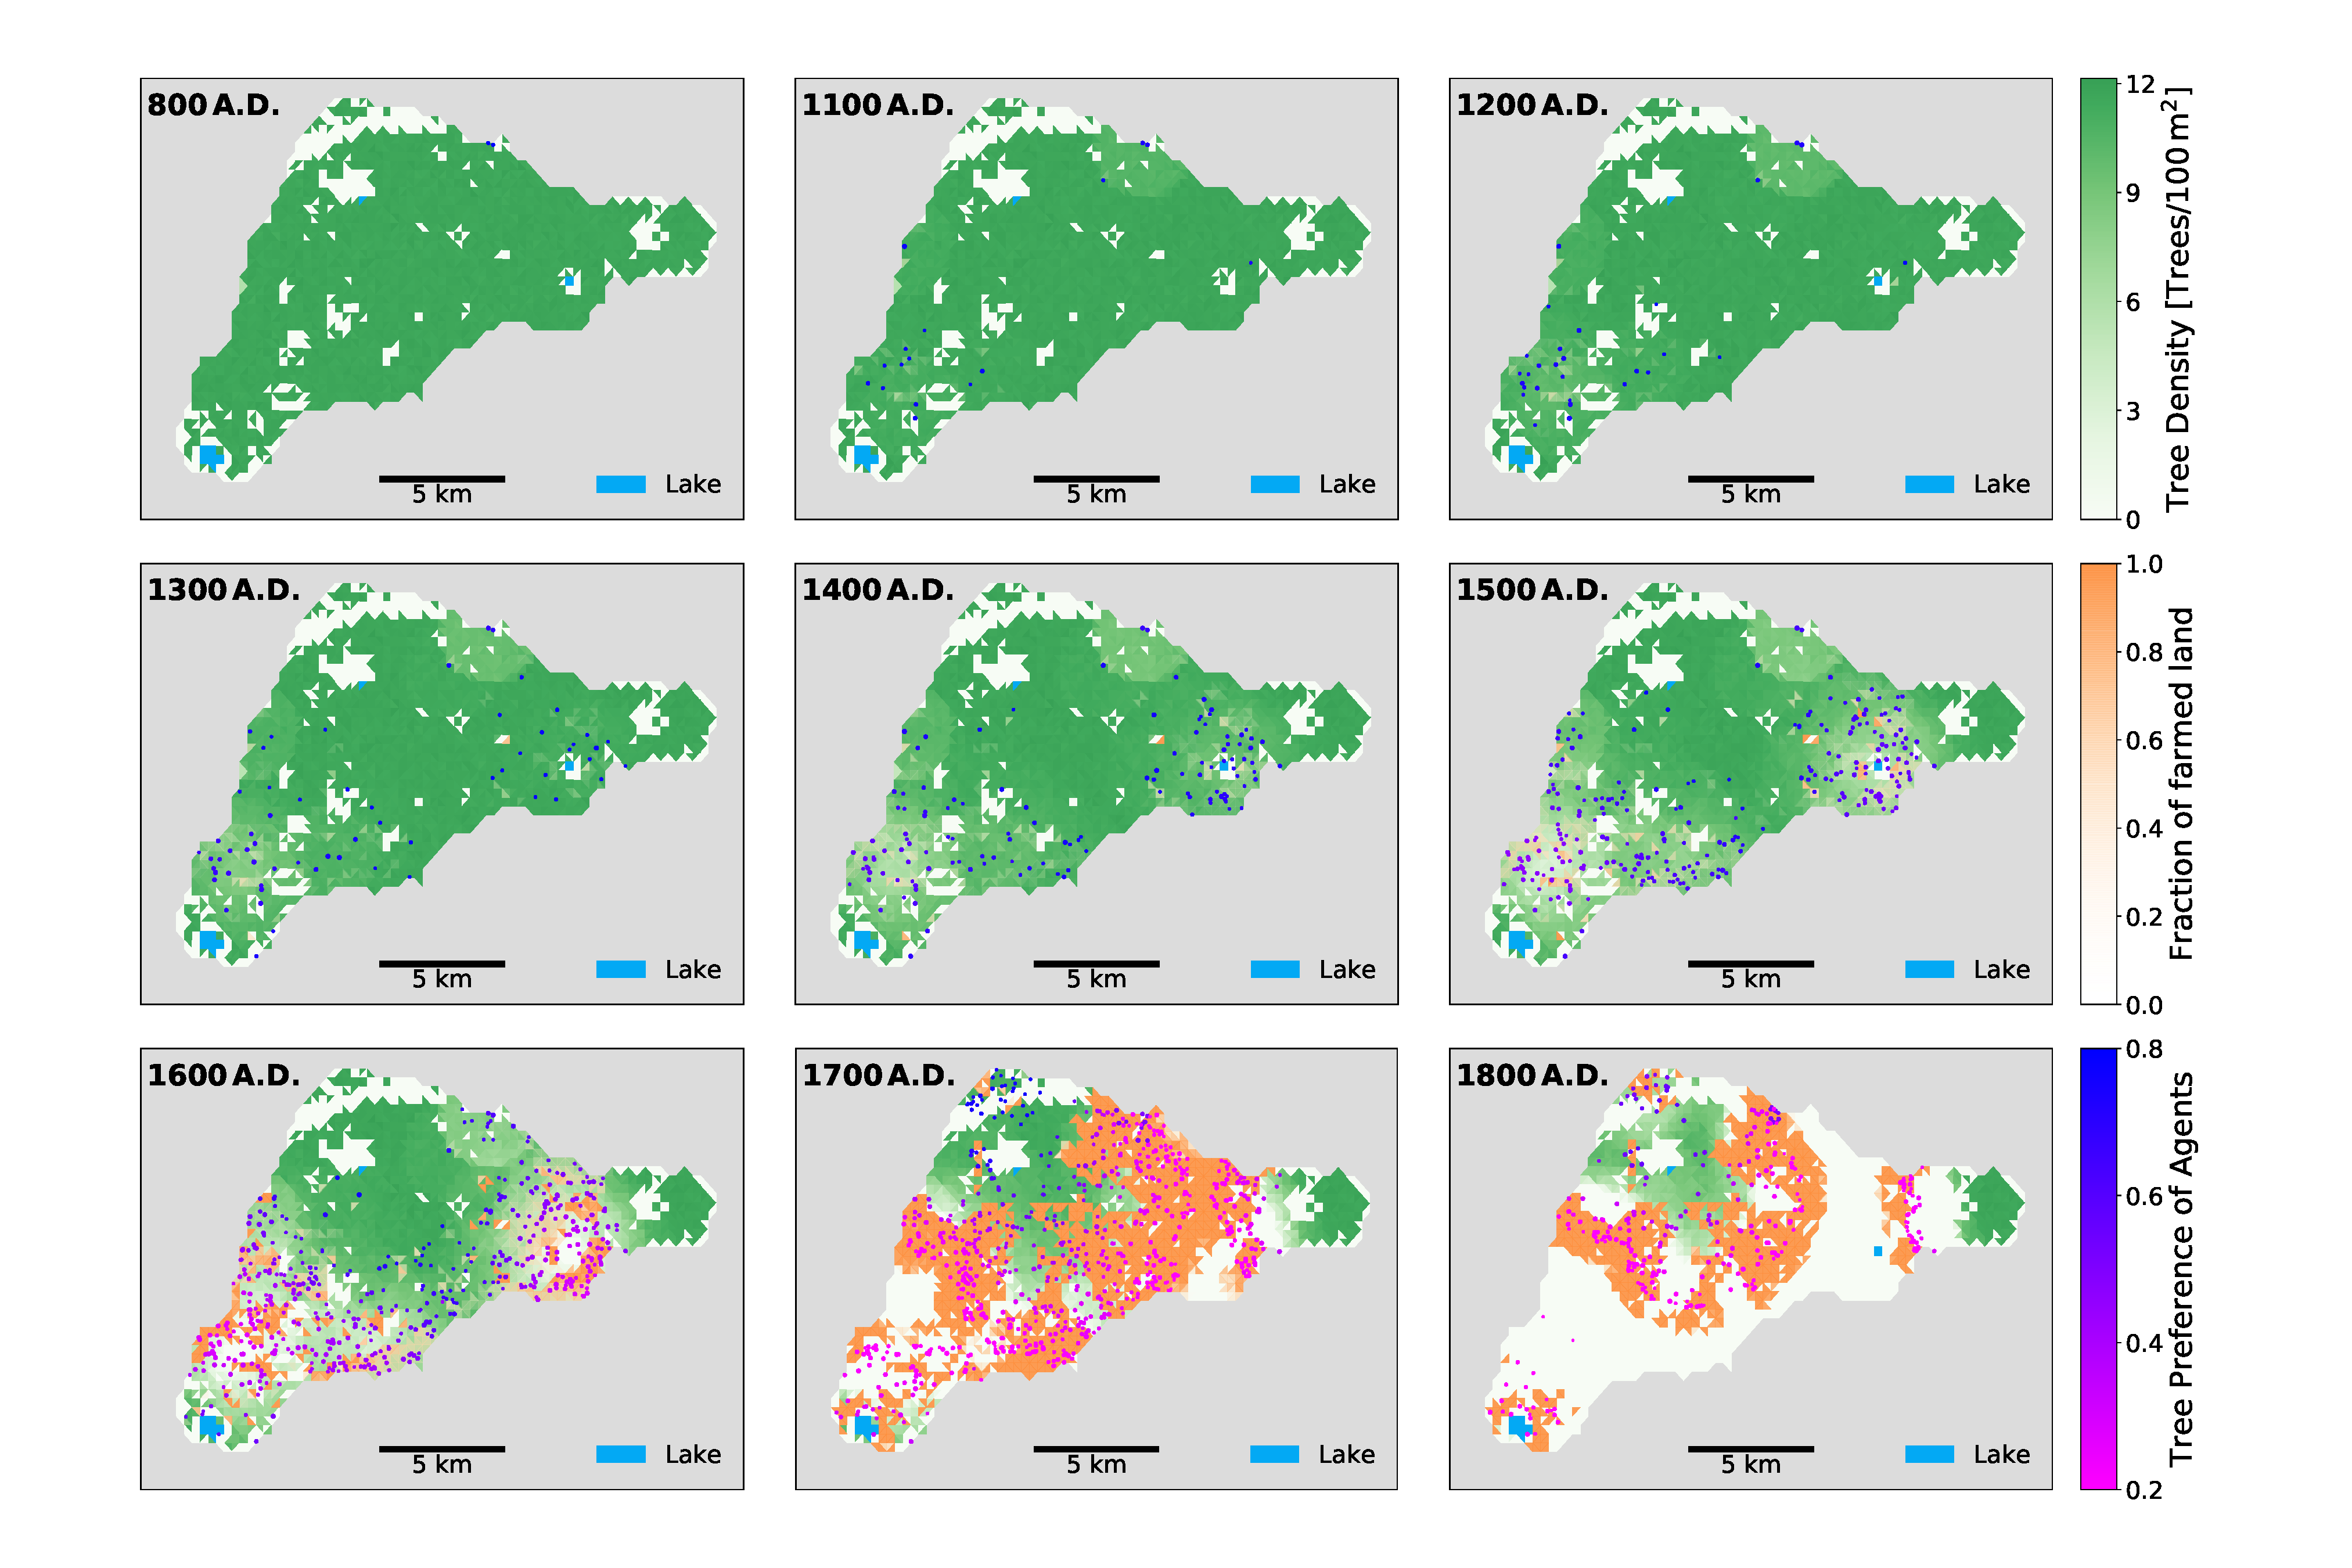
\includegraphics[width=1.0\linewidth]{images/Results/Standard/Rull2020_Comparison_seed3}
	\caption{The spatial patterns of for snapshots at 9 different times.  }
	\label{fig:STDrull}
\end{figure}


\begin{figure}
	\centering
	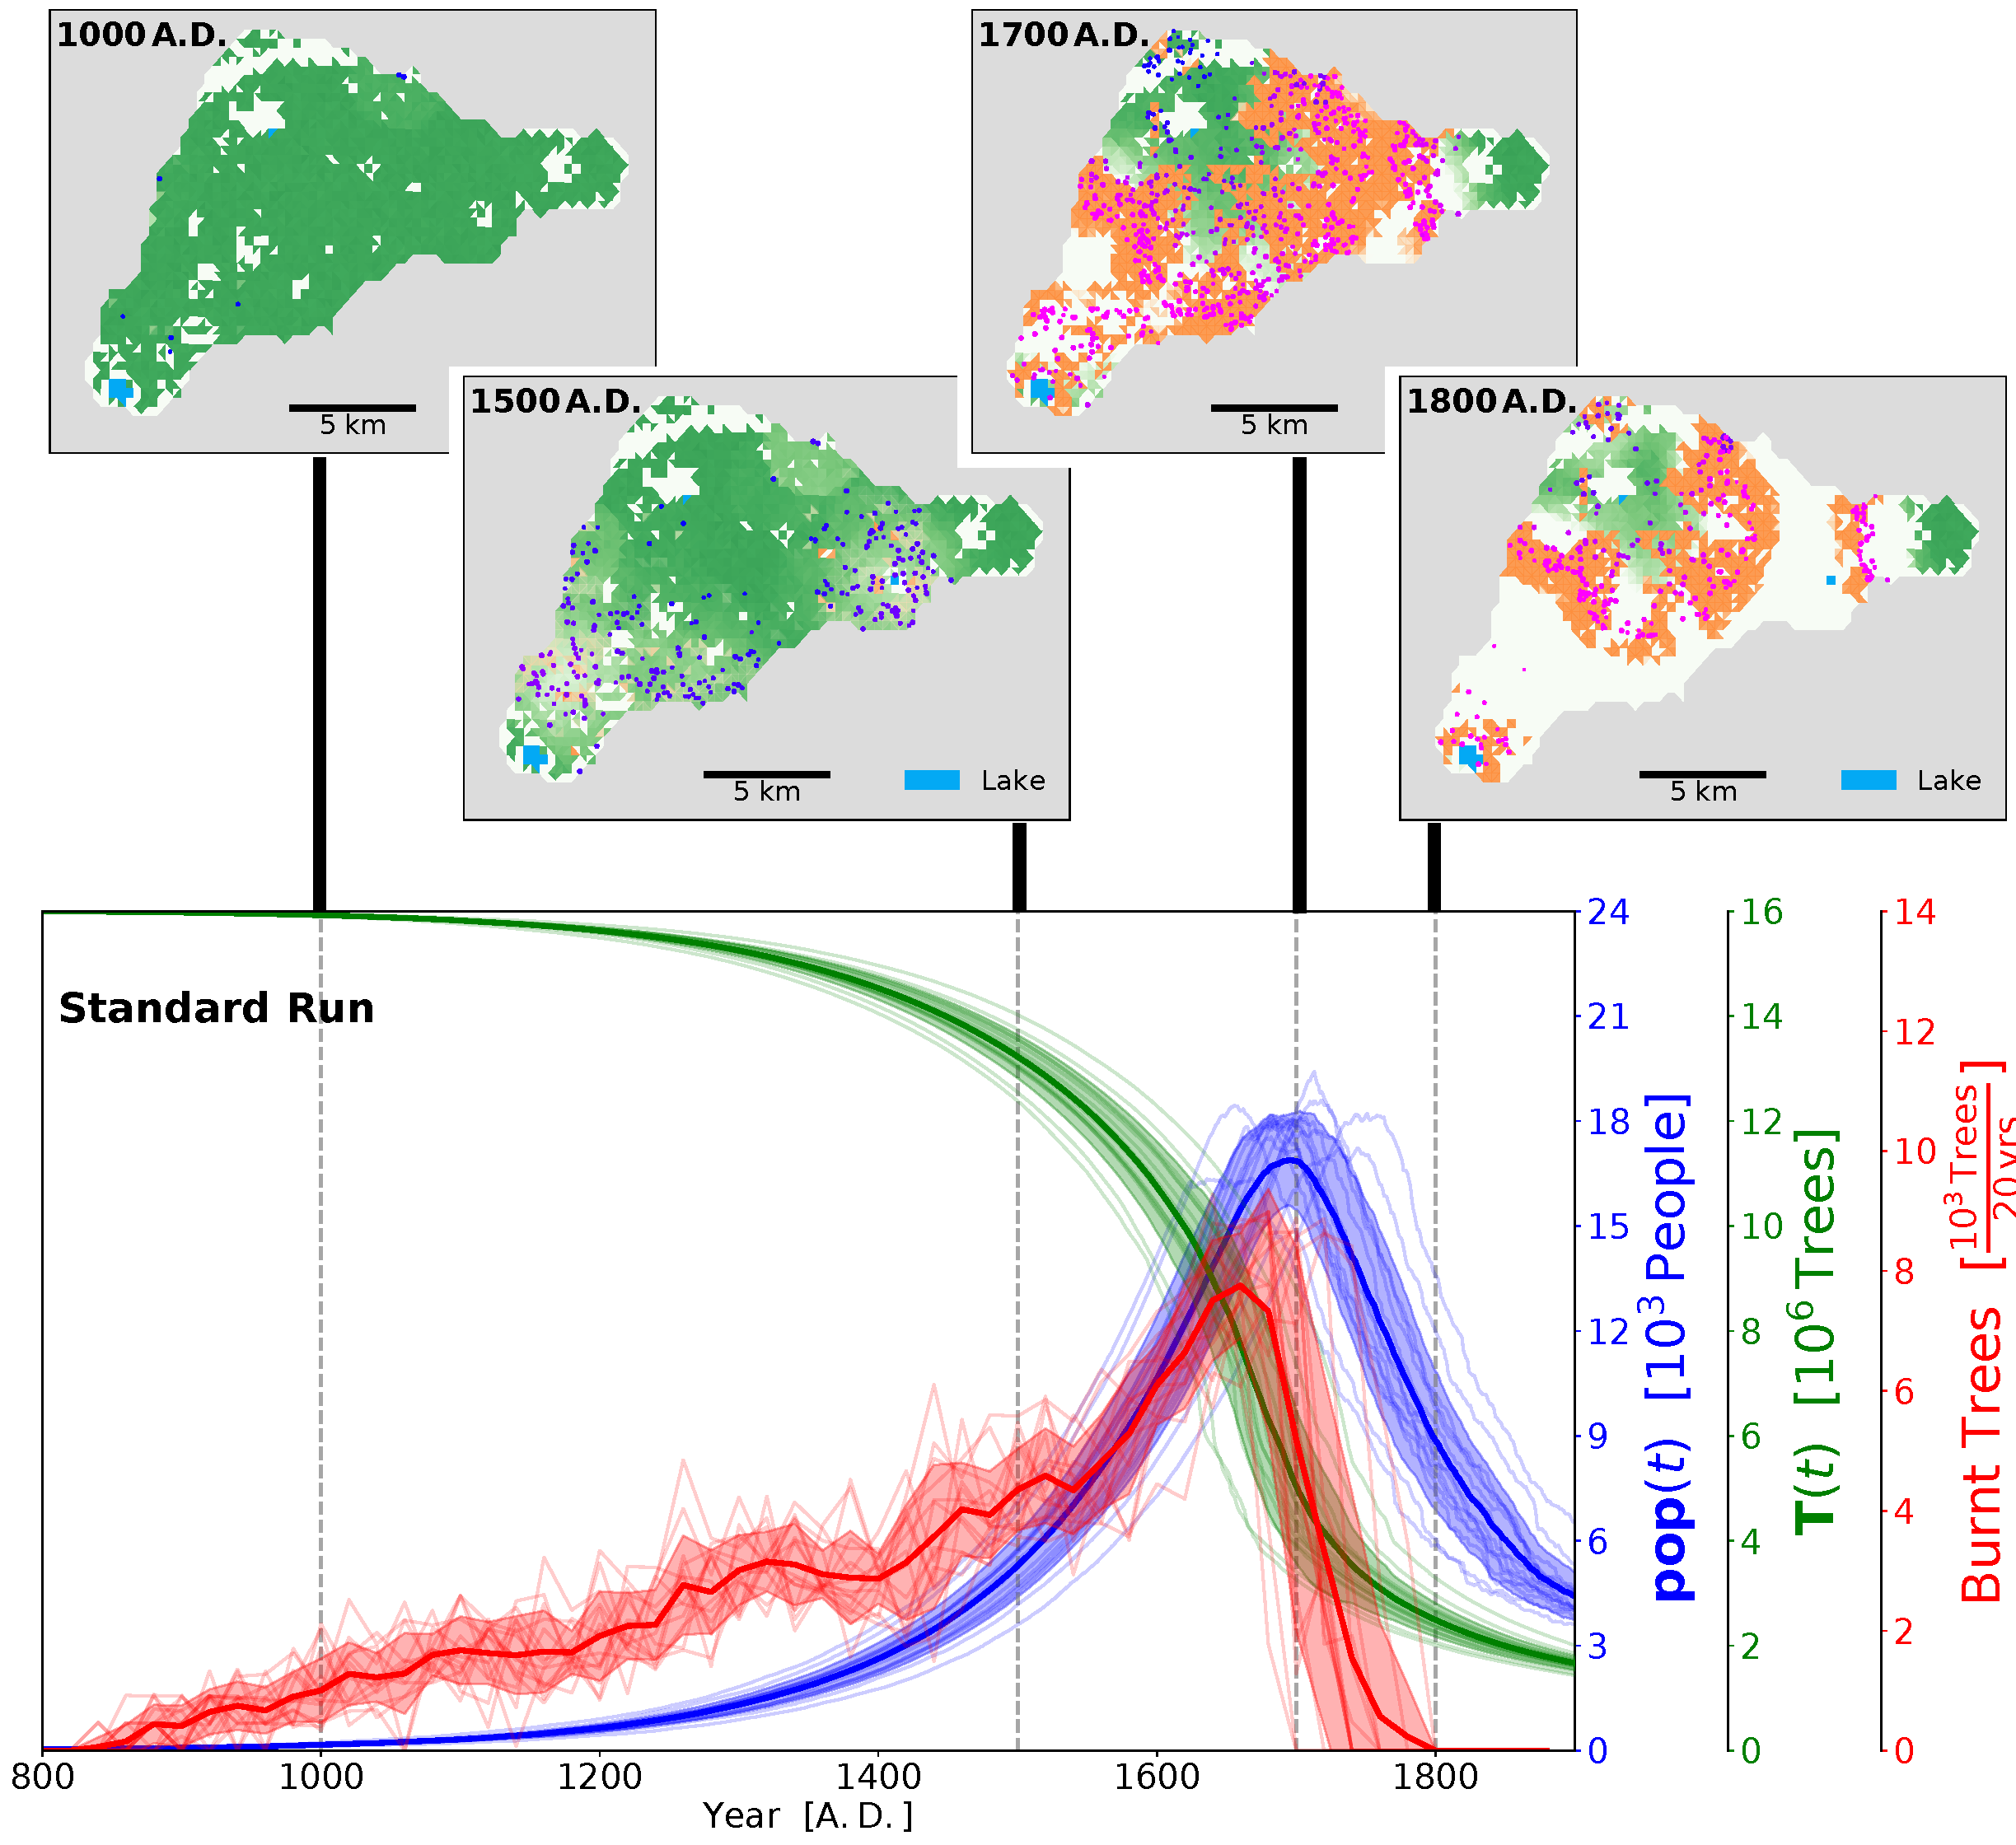
\includegraphics[width=1.0\linewidth]{images/Results/Standard/EnsembleStatistics+Panels}
	\caption{Dynamics of aggregate population size, trees, and burnt trees with standard setting of parameters. Five different realisations are used to obtain the ensemble mean and standard deviation (shaded area). The panels above show the spatial distribution of trees, farming and agent settlements with their tree preferences for one of these realisations (with the same scale as in Figure \ref{fig:STDrull}). }
	\label{fig:STDstats}
\end{figure}
%The dynamics of population size $\mathbf{pop}(t)$, total number of trees $\mathbf{T}(t)$ and amount of burnt trees in a 20 year time period) are shown in Figure \ref{fig:STDstats}. 
%For the first $850\, {\rm yrs}$ after arrival, the population grows exponentially.
%Then, around $1650\, {\rm A.D.}$ the dynamics change significantly, leading to a significant population size reduction after $1750\, {\rm A.D.}$.
%The rate of population size decrease is ....\TODO (i.e.\ the number of $g(H_{\rm i}(t))$ for agents $i$ and $t>1750\, {\rm A.D.}$ is on average ... \TODO.).


%
%We can look 
%Figure \ref{fig:app:treefillfarmfillmoves} 

\section{Different theories}
Statistics Plots for a
\begin{itemize}
	\item Run with low N fixation (instead of high)
	\item Run with tree regeneration and high N fixation
	\item Run with tree regeneration and low N fixation
\end{itemize}
In the making

\section{Different Tree Preference Functions, i.e.\ Agent Adaption}
\begin{itemize}
	\item Runs with $f_{\rm Tree \ Pref}$ delayed, careful, logistic.
\end{itemize}
I don't know yet if this makes any difference to the standard run and what difference. So we'll see.

Tree, Burn, Pop TPREF!!!


\section{A less resilient society}
Run with a larger shape parameter of $g(H_{\rm i})(t)$.
I don't know yet if this makes any difference to the standard run and what difference. So we'll see.
I assume that the turning point of growing population to decreasing population size happens earlier. Maybe I'll just show the statistics plot.


\section{Senstivity Analysis of some uncertain parameters}
$r_{\rm T}$, $r_{\rm F}$,
$T_{\rm Req, pP}$

\section{Three different decision making processes}
\begin{itemize}
	\item Standard setting, $\gamma=20$, $\alpha=(0.2,0.2,0.2,0.2,0.2)$.
	\item `Only resource availability matters for moving decision' setting, $\gamma=20$, $\alpha=(0, 0, 0, 0.5,0.5)$.
	\item Hopping agents, that move to a random spot with uniform probability over the island, $\gamma=0$, $\alpha=$ doesn't matter.
\end{itemize}
Results not yet known. I guess I'll describe qualitatively what happens to the spatial patterns. 
If the aggregate dynamics change, this would of course be a big, big result and I would focus on that.


\section{Perhaps, if I have time: Regional Dynamics}
Adjust the statistics plot of total population dynamics to looking at a few hand-defined regions and the plot the aggregate dynamics of them separately. 

\section{Fires}
Plot the distribution of fires on the map over time. 
I imagine a map in which the color determines the timing of fires in each cell. 
I'm not sure yet how to do this exactly since fires in any cell occur at multiple times. Maybe I'll take the first occurence. We'll see.



\chapter{Discussion and Conclusion}
